\chapter{Playing Sound}

\label{Chapter:Playing-Sound}
\lhead{\emph{Playing Sound}}

Sound playing implemented using midi output in our application 

Technically, a piece of music can be treated as a sequence of notes. In our model, a note is described by (pitch, start time, end time).
The pitch format here is different from the pitch format in the rendering engine, which use (step, octave) to describe a pitch.

\section{Pitch Conversion}
We tell the midi output server the notes' pitch by a number ranged from 0 to 255. The standard sound A4, with pitch 440Hz, is represented by 
value 69 in the midi protocol. With this knowledge, we can convert the (step, octave) pair into the midi pitch level by the formula:
\verb|pitchLevel = index('C D EF G A B', step) + octave * 12 - 48 + 60|. Here the ``index(list, element)'' function is used to locate the 
element in the list. For example, index(`C D EF G A B', `C') = 0, index(`C D EF G A B', `E') = 4.

\section{Time Conversion}
Usually, under the musical context, the unit of time is beat. For example, when the time signature is 3/4, it means there are 3 beats in each following
measure and the beat type is quarter beat. To convert to real world time, tempo is needed. Tempo tells us how many beats are there in one minute.
Suppose we have a note with duration equals to $t_d$, and tempo equals to $k$. Then the real world duration can be calculated by:
\[
t_d' = \frac{60 t_d}{k}
\]
The result unit is in seconds. Using this formula, we can accumulate the durations
to get the real world time relative to the beginning of each measure for each note.  

There is another element that can affect the duration of a note's duration. They 
are dots. With a single dot, the duration of a note is multiplied by $1.5$. However, 
with 2 dots, the duration is not multiplied by $1.5^2$. Instead, the result duration 
will be $t_d * (1 + \frac{1}{2} + \frac{1}{2^2})$, where $t_d$ is the origin duration.
Similarly, with $n$ dots, the converted duration will be:
\[
    t_d' = t_d \left(1 + \frac{1}{2} + \frac{1}{2^2} + \frac{1}{2^3} + \cdots + \frac{1}{2^n}\right)
         = t_d \left(2 - \frac{1}{2^n}\right)
\]

\section{Note Sequencing}
To get the final sequence of notes, we need to resolve the repeats in a musical score. At first,
all measures are chained together by in the order of their number. When we start to read a score, 
imagine the there is a cursor put at the beginning of the first measure. As we continue to read,
this cursor starts to move forward. When a end of repeat is encountered, the cursor need to jump back
to the corresponding start of repeat. When this repeat is encountered again, it should be ignored.
An example is illustrated by Figure \ref{fig:repeat-simple}. Sometimes there may be endings come along
with the repeat, this is illustrated by the example in \ref{fig:repeat-with-endings}. Other kinds of repeat
exists such as D.C.al Find(da capo al fine), etc. We will not discuss them here.

\begin{figure}[h]
    \centering
    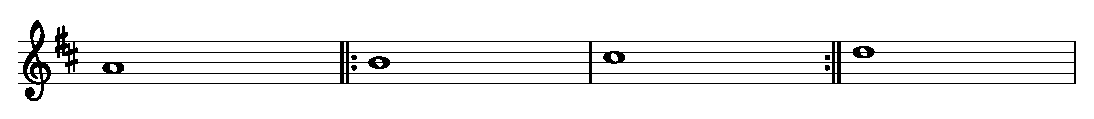
\includegraphics[width=\textwidth]{Figures/repeat-simple.eps}
    \caption{An example for typical repeat.}
    \label{fig:repeat-simple}
    \startdescription
    The read order should be 1,2,3,2,3,4.
\end{figure}

\begin{figure}[h]
    \centering
    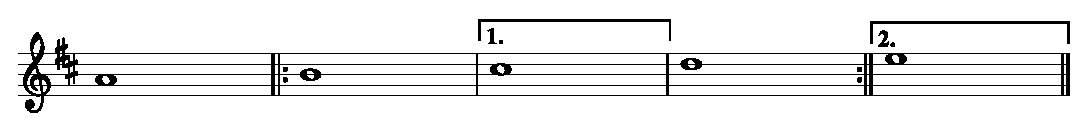
\includegraphics[width=\textwidth]{Figures/repeat-with-endings.eps}
    \caption{An example for repeat with endings.}
    \label{fig:repeat-with-endings}
    \startdescription
    The read order should be 1,2,3,4,2,5.
\end{figure}

% XXX: The flatten algorithm.

\section{Putting All Together}
The midi protocol support two types of event: note\_on and note\_off. We tell the midi server to
start playing a sound with note\_on(pitch, volume, channel) and use note\_off(pitch, volume, channel) to stop
the corresponding sound later. To work with the midi server, we need to convert the node sequence to note events.
Each note will generate exactly two events, one note\_on event and one note\_off event.

In our implementation, each event is described by (event\_type, time, note). To convert from notes to events, we first
generate $2n$ events from the $n$ notes. Then, the events are sorted by their time. Note that there maybe some different
events have the same time. In this case, we use the event type as the comparison key. More specifically, the note\_off event is considered ``less'' than the note\_on event. Otherwise, we are not able to play consecutive notes with same pitch.

The sound playing algorithm is shown in Algorithm \ref{algo:sound-playing}. To make it sound more fluently, we use an extra thread to run the code with implementing algorithm.

\begin{algorithm}
    \caption{Algorithm for Sound Playing} \label{algo:sound-playing}
    \begin{algorithmic}
        \Procedure{play\_sound}{events}
            \Require events sorted by (time, event\_type).
            \State $ t \gets 0$ \Comment{Current time}
            \For{ event $\in$ events}
                \State $ \Delta t \gets \mathrm{event.time} - t$
                \State sleep($\Delta t$)
                \State level $\gets$ convert\_pitch\_level(note.pitch)
                \If {event.type is note\_on}
                    \State note\_on(level, 127, 1)
                \Else
                    \State note\_off(level, 127, 1)
                \EndIf
            \EndFor
        \EndProcedure
    \end{algorithmic}
\end{algorithm}
